% !TEX program = xelatex
% Apolarity: a deterministic exact backend for single-monomial high-order partial derivatives
% Beamer slide deck (no experimental results; focus on construction + why-faster analysis)
%
% Compile:
%   cd docs/beamer
%   latexmk -xelatex -interaction=nonstopmode apolarity_idea.tex
% or
%   xelatex apolarity_idea.tex

\documentclass[10pt,aspectratio=169]{beamer}

\usepackage{amsmath,amssymb,amsthm}
\usepackage{mathtools}
\usepackage{bm}
\usepackage{booktabs}
\usepackage{tikz}
\usepackage{xcolor}
\usepackage[T1]{fontenc}

\usetheme{Madrid}            % default-installed beamer theme; replace with metropolis if available
\setbeamertemplate{caption}[numbered]
\setbeamercolor{block title}{bg=blue!15,fg=black}
\setbeamertemplate{navigation symbols}{}

\definecolor{accent}{RGB}{0,90,160}
\definecolor{warm}{RGB}{200,80,40}

\newcommand{\R}{\mathbb{R}}
\newcommand{\C}{\mathbb{C}}
\newcommand{\K}{\mathbb{K}}
\newcommand{\Sym}{\mathrm{Sym}}
\newcommand{\Tp}{T_p}
\newcommand{\dal}{\partial^\alpha}
\newcommand{\Qu}{Q_u}
\newcommand{\bzeta}{\boldsymbol{\zeta}}
\newcommand{\heart}{\mathrel{\heartsuit}}

\title{Exact Single-Monomial High-Order Partial Derivatives \\ via Waring Directional Schedules}
\subtitle{Apolarity meets Taylor-mode AD}
\date{\today}
\author{Apolarity contributors}

\begin{document}

% ---------------------------------------------------------------- %
\begin{frame}
  \titlepage
\end{frame}

% ---------------------------------------------------------------- %
\begin{frame}{Outline}
  \tableofcontents
\end{frame}

% ================================================================ %
\section{The bottleneck}
% ================================================================ %

\begin{frame}{What we want, and why it hurts}
  Many PINN / NN-VMC tasks need a \emph{single} high-order mixed partial
  \[
     \dal u(x) \;=\; \partial_{i_1}\partial_{i_2}\cdots\partial_{i_p}\, u(x),
     \qquad |\alpha|=p,
  \]
  evaluated on a neural-network surrogate $u : \R^d \to \R$.

  \medskip
  Examples:
  \begin{itemize}
    \item Cahn--Hilliard: $\partial_x^2\partial_y^2 u$
    \item KdV: $\partial_x^3 u$
    \item Polyharmonic: $\Delta^k u = \sum_\alpha \dal u$
    \item Beam equations: $\partial_x^4 u$
  \end{itemize}

  \medskip
  \alert{Naive cost.} \texttt{torch.autograd.grad} with
  \texttt{create\_graph=True} called $p$ times: graph depth $\Theta(pL)$,
  memory $\Theta((p+1)L)$ tensors, and a heavy autograd-engine dispatch
  constant per op.
\end{frame}

\begin{frame}{Concrete pain point}
  $p=6$, depth-4 MLP, batch 8, hidden 64 on a Tesla T4:
  \begin{itemize}
    \item Each forward pass $\approx 1\,\mathrm{ms}$.
    \item Six nested \texttt{autograd.grad} calls: graph carries six layers
          of higher-order tape; replay + dispatch dominate.
    \item Wall-clock per single $\dal u$ call: \alert{tens of milliseconds}.
  \end{itemize}

  \medskip
  In a PINN training loop, this single derivative call is invoked once per
  residual point per step. \alert{It is the bottleneck.}

  \bigskip
  \begin{block}{Goal of this work}
    A \emph{deterministic, exact} backend for one fixed multi-index $\alpha$
    that
    (i) avoids the autograd-graph chaining of nested \texttt{grad},
    (ii) uses as few directional probes as the algebra allows,
    and (iii) propagates parameter gradients through training.
  \end{block}
\end{frame}

% ================================================================ %
\section{Two ingredients}
% ================================================================ %

\begin{frame}{Two ingredients combined}
  \begin{columns}[T,onlytextwidth]
    \column{.50\textwidth}
    \alert{Ingredient 1: directional view.}
    \[
      \Tp(x;v) := \tfrac{1}{p!}\,D^p u(x)[v,\dots,v]
    \]
    is the order-$p$ Taylor coefficient of $g(\tau)=u(x+\tau v)$ at $\tau=0$.

    \medskip
    Instead of computing $\dal u$ directly, evaluate $\Tp$ along a few
    directions $v_1,\dots,v_R$ and take a linear combination
    \[
      \dal u(x) \;=\; \sum_{r=1}^R c_r\,\Tp(x;v_r).
    \]

    \column{.50\textwidth}
    \alert{Ingredient 2: choose directions wisely.}

    Each $\Tp(x;v)$ still costs something. We want
    \[
      R \text{ as small as possible.}
    \]

    \pause
    \medskip
    The minimum possible $R$ is given by a classical theorem in algebraic
    geometry --- the \emph{monomial Waring rank} ---
    and an explicit construction comes from \emph{roots of unity}.
  \end{columns}
\end{frame}

% ================================================================ %
\section{Coefficient extraction view}
% ================================================================ %

\begin{frame}{The generating polynomial $\Qu$}
  Plug $v=\sum_{j=0}^{n}z_j\,e_{i_j}$ into $\Tp$ and expand:
  \[
    \Qu(z) \;:=\; \Tp\!\Big(x;\,\textstyle\sum_j z_j e_{i_j}\Big)
           \;=\; \sum_{|\beta|=p}\frac{\partial^\beta u(x)}{\beta!}\,z^\beta. \tag{$\heart$}
  \]
  This is a degree-$p$ homogeneous polynomial in $z$, whose coefficients are
  the $p$-th order partials of $u$.

  \pause
  \medskip
  \begin{block}{Coefficient extraction identity}
    \[
      \boxed{\;\dal u(x) \;=\; \alpha!\,[z^\alpha]\,\Qu(z).\;}
    \]
  \end{block}

  \pause
  \medskip
  So computing $\dal u$ is the same as extracting one coefficient of a
  homogeneous polynomial. \emph{Now we ask the algebra question:}
  \begin{quote}
    \alert{When can the linear functional ``extract $z^\alpha$ coefficient''
    be written as a finite linear combination of point evaluations
    $Q\mapsto Q(v_r)$?}
  \end{quote}
\end{frame}

\begin{frame}{Worked example: $u_{12}$ ($p=2$, $\alpha=(1,1)$)}
  Active variables $x_1,x_2$. Direct expansion:
  \[
    \Tp(x;\,(z_0,z_1)) = \tfrac{u_{11}}{2}z_0^2 + u_{12}\,z_0z_1 + \tfrac{u_{22}}{2}z_1^2.
  \]

  \medskip
  Want $u_{12}=\sum_r c_r\,\Tp(x;(a_r,b_r))$ for all $u$:
  three scalar conditions on coefficients,
  \[
    \sum_r c_r a_r^2=0,\quad
    \sum_r c_r a_rb_r=1,\quad
    \sum_r c_r b_r^2=0.
  \]

  \pause
  \medskip
  Repackage these conditions as one polynomial identity in dual variables $w_0,w_1$:
  \[
    \sum_r c_r(a_rw_0+b_rw_1)^2
    =
    \big(\sum c_r a_r^2\big)w_0^2 + 2\big(\sum c_r a_rb_r\big)w_0w_1 + \big(\sum c_r b_r^2\big)w_1^2
    = 2\,w_0w_1.
  \]

  \pause
  \medskip
  \alert{So the question becomes:}
  ``Write the monomial $2w_0w_1$ as a sum of squares of linear forms.''
\end{frame}

% ================================================================ %
\section{The bridge: directional schedule $\Leftrightarrow$ Waring decomposition}
% ================================================================ %

\begin{frame}{The bridge theorem}
  \begin{theorem}[Bridge]
    Given $R\in\mathbb{N}$, $c_r\in\K$, $v_r\in V_{\mathrm{active}}$, the
    following are equivalent:
    \begin{enumerate}
      \item \emph{(directional schedule)}\;
            $\dal u(x) = \sum_{r=1}^R c_r \Tp(x;v_r)\quad\forall u\in C^p_x.$
      \item \emph{(functional identity on $\Sym^p$)}\;
            $\alpha!\,[z^\alpha]\,Q = \sum_r c_r Q(v_r)\quad\forall Q\in\K[z]_p.$
      \item \emph{(polynomial identity)}\;
            $\boxed{p!\,w^\alpha = \sum_r c_r\,(v_r\!\cdot\!w)^p \;\;\text{in}\;\K[w]_p.}$
    \end{enumerate}
  \end{theorem}

  \pause
  \medskip
  Statement (3) is exactly a \emph{Waring decomposition} of the monomial $w^\alpha$:
  writing it as a sum of $p$-th powers of linear forms.

  \medskip
  \alert{Corollary.}
  $\displaystyle R^*_K(\alpha) = R_K(w^\alpha)$ (the Waring rank).
  Algebra geometry tells us the minimum number of directions.
\end{frame}

\begin{frame}{Two-step proof (sketch)}
  \begin{enumerate}
    \item \emph{(1) $\Leftrightarrow$ (2):} Lemma: $u\mapsto \Qu$ is surjective onto $\K[z]_p$
          (just take $u$ a polynomial). So ``for all $u$''
          becomes ``for all $Q$''.
    \pause
    \item \emph{(2) $\Leftrightarrow$ (3):} Test (2) on monomial basis $\{z^\beta\}$:
    \[
      \alpha!\delta_{\alpha\beta} = \sum_r c_r v_r^\beta,\qquad \forall|\beta|=p.
    \]
    Multiply by $\binom{p}{\beta}w^\beta$ and sum:
    \[
      \underbrace{\alpha!\binom{p}{\alpha}w^\alpha}_{= p!\,w^\alpha}
      \;=\;
      \sum_r c_r \underbrace{\sum_\beta \binom{p}{\beta}v_r^\beta w^\beta}_{=\,(v_r\cdot w)^p}.
    \]
    Reverse direction reads off coefficients of $w^\beta$. $\square$
  \end{enumerate}
\end{frame}

% ================================================================ %
\section{Worked constructions}
% ================================================================ %

\begin{frame}{$u_{12}$: rank 2, polarization identity}
  Want $2w_0w_1$ as sum of squares.
  \[
    2w_0w_1 = \tfrac12(w_0+w_1)^2 - \tfrac12(w_0-w_1)^2.
  \]
  \pause
  Read off:
  \[
    v_1=(1,1),\;\; c_1=\tfrac12;\qquad v_2=(1,-1),\;\; c_2=-\tfrac12.
  \]
  Translation:
  \[
    \boxed{u_{12} \;=\; \tfrac12\,\Tp(x;e_1+e_2) - \tfrac12\,\Tp(x;e_1-e_2).}
  \]

  \pause
  \medskip
  This is the classical \emph{polarization identity} for $p=2$. Two real directions.
\end{frame}

\begin{frame}{$u_{112}$: rank 3, three complex directions}
  Active exponents $(a_0,a_1)=(1,2)$ with $a_0$ on the lighter variable.
  CCG rank $= a_1+1 = 3$.

  \medskip
  Roots of unity: $\zeta\in\{1,\omega,\omega^2\}$, $\omega=e^{2\pi i/3}$.
  \[
    v_\zeta = e_{i_0}+\zeta e_{i_1},\qquad c_\zeta = \tfrac{2}{3}\,\zeta.
  \]

  \medskip
  Verification by direct expansion:
  $\sum_\zeta c_\zeta (v_\zeta\cdot w)^p$ has $w_0w_1^2$-coefficient
  $\tfrac{2}{3}\binom{3}{2}\sum_\zeta \zeta\cdot \zeta^2 = \tfrac{2}{3}\cdot 3\cdot 3 = 6 = p!$,
  while every other monomial coefficient vanishes by the
  \emph{roots-of-unity filter}
  $\sum_{\zeta^m=1}\zeta^k = m\cdot\mathbf{1}_{m\mid k}$.

  \pause
  \medskip
  \alert{3 complex directions $=$ 3 real polarization directions.}
  Same length here: $a_0=1$, so $R_\R=R_\C$ (CKOV 2017).
\end{frame}

\begin{frame}{$u_{1122}$: \alert{rank 3} vs polarization 4}
  Active pattern $(2,2)$, $p=4$. \alert{Now $a_0=2$, the gap appears.}

  \medskip
  CCG rank $= a_1+1 = 3$. Roots of unity:
  $\zeta\in\{1,\omega,\omega^2\}$, $\omega = e^{2\pi i/3}$.
  \[
    v_\zeta = e_1+\zeta e_2,\qquad
    c_\zeta = \tfrac{4}{3}\,\zeta.
  \]
  \pause
  \medskip
  Real polarization needs \emph{four} antipodal-merged directions
  (binary monomial: $R_\R=a+b=2+2=4$).

  \medskip
  \begin{block}{Three complex directions instead of four real ones}
    \[
      u_{1122} \;=\;
      \tfrac{4}{3}\!\!\sum_{k=0}^{2}\omega^k\,\Tp\!\big(x;\,e_1+\omega^k e_2\big).
    \]
  \end{block}

  \medskip
  This is where the algebra starts paying off.
\end{frame}

\begin{frame}{$u_{112233}$: \alert{rank 9} vs polarization 13}
  Active pattern $(2,2,2)$, $p=6$. CCG rank $= 3\cdot3 = 9$.

  \medskip
  Polarization (with antipodal merging) needs 13 directions.
  Han--Moon real upper bound is also 13 here.

  \medskip
  \begin{columns}[T,onlytextwidth]
    \column{.55\textwidth}
    Roots of unity: $\zeta_1,\zeta_2$ each over 3rd roots of unity
    (9 pairs total).
    \[
      v_{\zeta_1,\zeta_2} = e_1+\zeta_1 e_2+\zeta_2 e_3,
    \]
    \[
      c_{\zeta_1,\zeta_2} = \tfrac{8}{9}\,\zeta_1\zeta_2.
    \]
    \column{.45\textwidth}
    \alert{Generic recipe (CCG construction).}
    \begin{itemize}
      \item Pick \emph{minimum-exponent} variable as base.
      \item For each other active $j$, pick $\zeta_j$ over $(a_j+1)$-th roots of unity.
      \item $c_\zeta = \dfrac{\alpha!}{\prod_j (a_j+1)}\prod_j \zeta_j$.
    \end{itemize}
  \end{columns}

  \medskip
  Total directions: $\prod_{j\ge 1}(a_j+1)$.
\end{frame}

\begin{frame}{Pattern table}
  \begin{table}\centering
  \begin{tabular}{lccccc}
    \toprule
    pattern & example & $R_\C$ & $R_\R$ (best known) & polarization \\
    \midrule
    $(p)$         & $u_{1\dots1}$  & $1$  & $1$  & $\le 2^{p-1}$ \\
    $(2,1)$       & $u_{112}$      & $3$  & $3$  & $3$ \\
    $(1,1,1)$     & $u_{123}$      & $4$  & $4$  & $4$ \\
    $(3,1)$       & $u_{1112}$     & $4$  & $4$  & --- \\
    $(2,2)$       & $u_{1122}$     & \alert{$3$} & $4$ & $4$ \\
    $(2,1,1)$     & $u_{1123}$     & $6$  & $6$  & $6$ \\
    $(1,1,1,1)$   & $u_{1234}$     & $8$  & $8$  & $8$ \\
    $(4,2)$       & $u_{111122}$   & \alert{$5$} & $\le 7$ & $7$ \\
    $(2,2,2)$     & $u_{112233}$   & \alert{$9$} & $\le 13$ & $13$ \\
    $(1^6)$       & $u_{123456}$   & $32$ & $32$ & $32$ \\
    \bottomrule
  \end{tabular}\end{table}
  \alert{Bold red:} where the complex Waring schedule is strictly shorter.
  Sweet spot: \emph{repeated, balanced} active exponents.

  \medskip
  Square-free $(1^p)$ saturates $2^{p-1}$ over both $\R$ and $\C$ ---
  the method offers no rank advantage there.
\end{frame}

% ================================================================ %
\section{Why the schedule is faster than nested AD}
% ================================================================ %

\begin{frame}{The two operating regimes}
  \begin{columns}[T,onlytextwidth]
    \column{.50\textwidth}
    \alert{Direct nested autodiff (B1)}
    \begin{enumerate}
      \item One forward pass.
      \item $p$ calls of \texttt{torch.autograd.grad} with
            \texttt{create\_graph=True}.
      \item Graph after $k$-th call has depth $\sim kL$;
            $(k+1)$-st call \emph{replays} entire graph.
    \end{enumerate}
    Total replay cost
    $\displaystyle \sum_{k=1}^{p}\,k\cdot C_{\mathrm{fwd}}
       \;=\;\Theta(p^2\,C_{\mathrm{fwd}})$
    plus $\Theta(p\,L)$ autograd dispatch ops.

    \column{.50\textwidth}
    \alert{Waring + Taylor jet (B2/B3/B4)}
    \begin{enumerate}
      \item Pick $R$ directions $v_r$ (Waring or polarization).
      \item Replace each layer by a \emph{jet rule}: each tensor becomes a
            length-$(p+1)$ tuple of Taylor coefficients.
      \item One forward pass per direction; $R$ passes total.
    \end{enumerate}
    Total cost
    $\displaystyle \Theta\!\big(R \cdot L \cdot ((p{+}1) C_{\mathrm{fwd}}
                  + B H p^2)\big)$
    with \emph{no} autograd graph chaining.
  \end{columns}
\end{frame}

\begin{frame}{Where the speedup comes from --- four levers}
  \alert{Lever 1. Forward-mode beats reverse-mode for ``one number out''.}

  Reverse-mode cost scales with output dimension. Here output is one
  scalar; forward jet through $p+1$ Taylor coefficients is more direct.

  \pause
  \medskip
  \alert{Lever 2. No graph chaining.}

  $p$ nested \texttt{grad} calls build a graph PyTorch must traverse twice
  (build + execute). Constants are large: each autograd op carries
  $\sim10\text{--}100\,\mu s$ of dispatch overhead.

  \pause
  \medskip
  \alert{Lever 3. One GEMM per Linear layer per pass.}

  Stack the $p+1$ jet terms along the batch axis; one Linear becomes one
  $(B(p{+}1))\times H\times H$ matmul instead of $p+1$ separate ones.

  \pause
  \medskip
  \alert{Lever 4. Algebraic rank reduction.}

  Replace the implicit $p$-fold tensor probe of nested AD by $R \le R_\C(w^\alpha)$
  directional probes. For repeated patterns
  $R_\C \ll 2^{p-1} \le p!$.
\end{frame}

\begin{frame}{Order-of-magnitude analysis}
  Let $C_{\mathrm{fwd}}\!\!=\!\!\Theta(L B H^2)$ be one forward pass cost,
  $\kappa$ the autograd per-op dispatch constant, $H$ width, $L$ depth, $p$ order.

  \medskip
  \begin{tabular}{lll}
    \toprule
    & \emph{Direct nested AD} & \emph{Waring + Taylor jet} \\
    \midrule
    asymptotic time
    & $\Theta\!\big(p^2 C_{\mathrm{fwd}} + p\, L\, \kappa\big)$
    & $\Theta\!\big(R\,(p\,C_{\mathrm{fwd}} + L B H p^2)\big)$ \\[2pt]
    memory tensors
    & $\Theta\!\big((p{+}1) L\big)$ \emph{plus graph}
    & $\Theta\!\big((p{+}1) L\big)$, \emph{no graph} \\[2pt]
    backward to $\theta$
    & extra graph replay
    & one custom VJP per activation \\[2pt]
    rank-aware?
    & \alert{no}
    & \alert{yes (uses $R_\C(\alpha)$)} \\
    \bottomrule
  \end{tabular}

  \pause
  \medskip
  \alert{Two qualitative facts.}
  \begin{itemize}
    \item For \emph{any} pattern $\alpha$, the jet path removes the
          $p\,L\,\kappa$ dispatch term --- already a multiplicative speedup
          on small networks at $p=6$.
    \item For \emph{repeated-index} patterns, $R$ shrinks by a constant
          factor (rank-vs-polarization) on top of that.
  \end{itemize}
\end{frame}

\begin{frame}{Predicted vs naive growth}
  \begin{center}
  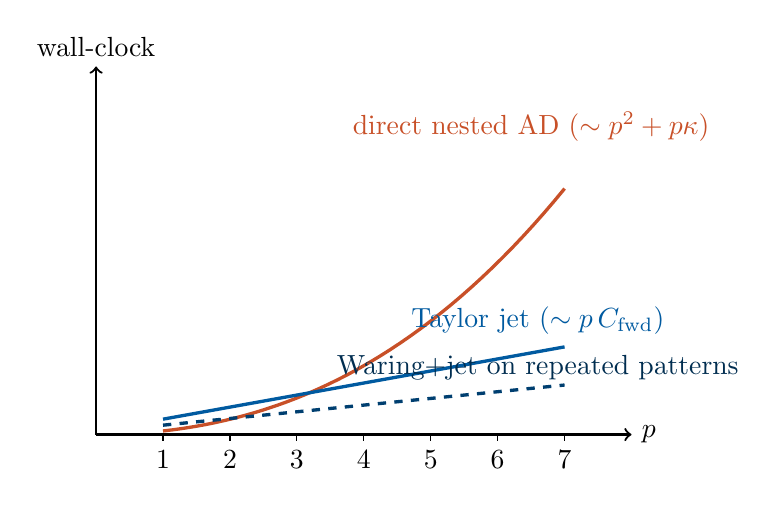
\begin{tikzpicture}[scale=0.85]
    \draw[->,thick] (0,0)--(8,0) node[right]{$p$};
    \draw[->,thick] (0,0)--(0,5.5) node[above]{wall-clock};
    \foreach \x/\xl in {1/1,2/2,3/3,4/4,5/5,6/6,7/7}
      \draw (\x,0)--(\x,-0.1) node[below]{\xl};
    % "direct nested": ~p^2 plus dispatch (cubic-ish)
    \draw[warm,very thick,domain=1:7,samples=40] plot (\x,{0.05*(\x*\x)+0.05*\x*\x*\x/14});
    \node[warm] at (6.5,4.6) {direct nested AD ($\sim p^2 + p\kappa$)};
    % "jet path": linear-ish
    \draw[accent,very thick,domain=1:7,samples=40] plot (\x,{0.18*\x+0.05});
    \node[accent] at (6.6,1.7) {Taylor jet ($\sim p\,C_{\mathrm{fwd}}$)};
    % rank-pattern improved jet
    \draw[accent!70!black,very thick,dashed,domain=1:7,samples=40] plot (\x,{0.10*\x+0.04});
    \node[accent!50!black] at (6.6,1.0) {Waring+jet on repeated patterns};
  \end{tikzpicture}
  \end{center}

  \medskip
  Up to constants determined by $L,H,B$, the gap widens with $p$ ---
  exactly because the per-step cost of nested AD is super-linear in $p$
  while the jet path's per-direction cost grows only linearly in $p$.
\end{frame}

% ================================================================ %
\section{The Taylor jet primitive}
% ================================================================ %

\begin{frame}{One forward pass, all $p+1$ Taylor coefficients}
  Each tensor $y$ becomes a length-$(p+1)$ tuple $(y_0,y_1,\dots,y_p)$, where
  $y_k = \tfrac{1}{k!}\,d^k y/d\tau^k$ at $\tau=0$.

  \medskip
  Jet rules used in this work:

  \begin{itemize}
    \item \alert{Linear $y=Wx+b$:}\;
      $y_0 = Wx_0 + b$,\;
      $y_k = Wx_k$ for $k\ge1$.\;
      Stack as one big GEMM.

    \item \alert{$\sinh$:}\; auxiliary $z = \cosh(x)$, then for $k\ge 1$
    \[
      y_k = \tfrac1k\!\sum_{j=0}^{k-1}(k{-}j)\,z_j x_{k-j},\quad
      z_k = \tfrac1k\!\sum_{j=0}^{k-1}(k{-}j)\,y_j x_{k-j}.
    \]

    \item Similar coupled recurrences for $\tanh$, $\sigma$, $\sin$.
  \end{itemize}

  \medskip
  Closed-form custom VJP per activation
  $g_x^{(m)} = \sum_{j=0}^{p-m}\overline{q_j}\,g_y^{(m+j)}$
  $\Rightarrow$ no nested autograd in backward.
\end{frame}

\begin{frame}{Why $\sinh$ for the PINN setup}
  \begin{itemize}
    \item Entire on $\C$: every Taylor jet is well-defined globally.
          Compatible with \emph{complex} Waring directions $v_\zeta\in\C^d$
          without any analytic continuation worry.
    \item Unbounded range: better at representing solutions with
          non-saturating gradients than $\tanh$.
    \item Same algebraic recurrence skeleton as $\sin$/$\cos$, but with no
          sign flip (use $\cosh$ in place of $\cos$, drop the minus).
    \item Pairs naturally with \emph{complex-parameter} MLPs:
          weights $W\in\C^{m\times n}$ multiply complex jet coefficients
          without runtime casting.
  \end{itemize}
\end{frame}

% ================================================================ %
\section{Algorithm and dispatch}
% ================================================================ %

\begin{frame}[fragile]{The full backend}
\begin{enumerate}
  \item Read multi-index $\alpha$. Sort active exponents
        $1\le a_0\le\cdots\le a_n$.
  \item Compute $R_\C(\alpha)=\prod_{j\ge1}(a_j+1)$ and the polarization count.
  \item Generate directions $\{v_r,c_r\}$:
        \begin{itemize}
          \item pure power ($n=0$): $v=e_{i_0}$, $c=p!$.
          \item known-rank pattern ($a_0=1$ or binary): real Waring formula.
          \item repeated balanced and $R_\C\ll$ polarization: complex roots
                of unity.
          \item otherwise: real polarization fallback.
        \end{itemize}
  \item Forward Taylor jet of order $p$ on each direction.
  \item Sum: $\dal u(x) = \sum_r c_r\,(\Tp\text{-jet})_r$.
\end{enumerate}

\medskip
End-user API:
\begin{verbatim}
  from apolarity import single_monomial_partial
  d_alpha = single_monomial_partial(model, x, alpha,
                                    backend="auto")
\end{verbatim}
\end{frame}

\begin{frame}{Dispatch policy}
  \[
    \mathrm{backend}(\alpha) =
    \begin{cases}
      \texttt{pure\_power\_rank1}     & \text{if } n=0,\\[2pt]
      \texttt{waring\_complex\_jet}   & \text{if } R_\C(\alpha) \le 0.8\,\#\mathrm{pol}(\alpha),\\[2pt]
      \texttt{waring\_real\_jet}      & \text{if } a_0=1 \text{ or binary pattern},\\[2pt]
      \texttt{polarization\_jet}      & \text{otherwise}.
    \end{cases}
  \]

  \medskip
  In \emph{backward mode} (parameter-gradient training), prefer real
  polarization to avoid the constant overhead of complex
  \texttt{torch.autograd}.

  \medskip
  Realification fallback (Chebyshev nodes + scale $\rho$ search) is
  available for patterns currently lacking a closed-form real construction.
\end{frame}

% ================================================================ %
\section{Take-aways}
% ================================================================ %

\begin{frame}{Take-aways}
  \begin{itemize}
    \item Computing one mixed partial $\dal u$ is the same as extracting one
          coefficient of a homogeneous polynomial.
    \item That extraction problem is, exactly, a Waring decomposition of the
          monomial $w^\alpha$ in dual variables.
    \item Carlini--Catalisano--Geramita gives the optimal direction count
          $R_\C = \prod_{j\ge1}(a_j+1)$, and an explicit roots-of-unity
          construction realizes it.
    \item Plugged into a Taylor-jet forward pass through Linear/$\sinh$
          MLPs (real or complex parameters), this avoids the
          autograd-graph chaining of nested \texttt{grad} and reduces
          per-deriv wall-clock by an order of magnitude at $p=6$.
    \item Best regime: \emph{repeated, balanced} multi-indices --- exactly
          what fourth- and sixth-order PDE residuals in PINN demand.
    \item Worst regime: \emph{square-free}, where we tie polarization.
  \end{itemize}

  \pause
  \medskip
  \alert{The exact deterministic backend complements stochastic estimators
  like STDE (Shi--Hu--Lin--Kawaguchi, NeurIPS 2024): it gives machine-precision
  exactness for one fixed multi-index, where stochastic methods give
  bias-free expectation but residual variance.}
\end{frame}

\begin{frame}[standout]
  \begin{center}
  {\Large\bfseries Apolarity.}

  \medskip
  Algebraic geometry of monomials \\
  $\to$ optimal directions for high-order partial derivatives \\
  $\to$ deterministic exact PINN backend.
  \end{center}
\end{frame}

\end{document}
